\documentclass[uplatex, twocolumn, 10pt]{jsarticle} % Underfull \vbox (badness 10000) 文書の見た目が悪いらしいが、解決方法がよく分からない

\usepackage[dvipdfmx]{graphicx} % 画像処理に関するやつ
\usepackage{latexsym} % 数学の記述や論文作成などで頻繁に使用されるらしいやつ
\usepackage{bmpsize} % フォントのサイズ
\usepackage{url} % urlを扱うときに必要
\usepackage{comment} % 複数行のコメントができるらしいけど、#でいい気がする
\usepackage{amsmath} % 数式を扱う上で必要
\usepackage{algorithm} % アルゴリズムの記述に使用
% 余白の調整
% \usepackage[top=25truemm,bottom=25truemm,left=20truemm,right=20truemm]{geometry}
\setlength{\textheight}{636pt}
\setlength{\textwidth}{453pt}

% 使い方の例:\Underline{これが下線で強調されるテキストです。}\endUnderline
\def\Underline{\setbox0\hbox\bgroup\let\\\endUnderline} 
\def\endUnderline{\vphantom{y}\egroup\smash{\underline{\box0}}\\}

% コードの表示やコンピュータのファイル名、変数名などを強調するのに便利らしい(ソースはchatgpt)
\newcommand{\ttt}[1]{\texttt{#1}}

%%%  文書の最初  %%%
\begin{document}


% =================  タイトル  ====================
% 別な書き方
% \title{\bf
% {\LARGE{Codeless Web Testing using Selenium and Machine Learning\\
% Seleniumと機械学習を用いたコードレスWebテスト} \\ 
% \Large{Duyen Phuc Nguyen, Stephane Maag\\
% ICSOFT 2020: 15th International Conference on Software Technologies, Jul 2020, Online, France.
% pp.51-60}
% }}
\title{Automatic Generation of Test Cases from Formal Specifications using Mutation Testing \\
    ミューテーションテストを用いた形式仕様からの\\テストケースの自動生成}
\author{R. J. Cajica, R. E. G. Torres and P. M. \'Alvarez\\
    2021 18th International Conference on Electrical Engineering,\\ Computing Science and Automatic Control (CCE),\\ 2021, pp.1-6\\
    doi: 10.1109/CCE53527.2021.9633118.\\\\ 訳: 高橋 朋弘}
\date{2025年6月6日(金)}
\maketitle

% =================  概要  ====================
\section*{概要} % \section*は章番号をつけない
複雑なソフトウェアシステムのテストでは、コード内のエラーを見つけ、システムの高い整合性を確保するために、何千ものテストケースを実行する必要がある。
そのため、テストタスクの自動化は不可欠である。
テストケースの実行は、事前条件と入力データの確立、出力データの観察、およびそれらの結果と特定のオラクルとの比較を伴う。
本研究では、以下の2つの貢献を示す。
テストケース生成器として粒子群最適化 (PSO: Particle Swarm Optimization) アルゴリズムを使用したこと。
また、SOFLを用いて、形式仕様に対しミューテーションテストを使用したことである。
形式仕様に対するミューテーションテストにより、より多くのミュータントを殺す新しいテストケースを発見することができる。
その結果として、より多くのエラーを検出可能なテストスイートの構築が期待できる。
入力 (テストケース) の値を生成するために、PSO アルゴリズムを適用する。
本研究では、ソフトウェアの例を用いて、提案するテストフレームワークの高い効率性を示す。

% =================  1.はじめに  ====================
\section{はじめに} % 1章
ソフトウェアテストは、あらゆるソフトウェア開発手法において不可欠なプロセスであり、自動化していない場合、システムの動作の評価を行う担当者に多大な時間と集中力を求める。
ソフトウェアテストの本質は、テスト対象となるソフトウェアの一連のテストケースを特定することである。
このテストケースを作成する方法の1つは、システム仕様を使用することである。
形式言語を用いて非形式な仕様を形式化することにより、コスト効率が高い方法で信頼性の高いシステムを構築できる。

本研究では、形式言語 SOFL で記述した仕様から、テストセットを生成するためのソフトウェアツールの開発について説明する。
本ツールでは、SOFL の述語仕様から拡張機能シナリオを作成する。
機能シナリオの各要素に対して、PSO アルゴリズムを用いて、各述語を満たすテストケースを生成する。
生成した各テストケースから、ミュータントのリストを作成する。
最後に、ミュータントリストの各ミュータントを使用して、テストケースを生成する。

% =================  2. 背景  ====================
\section{背景}
\label{sec:background}
\subsection{ソフトウェアテスト}
ソフトウェアテストは、ソフトウェアエンジニアリングの一分野であり、ソフトウェアの仕様に基づいて、ソフトウェアの品質を評価する役割を担う。
そのためには、テストスイートとテストオラクルを生成する必要がある。
テストオラクルは、システムの動作が正しいかどうかを判断する役割を担う。

ソフトウェアテストに関する研究は、テストケースおよびテストオラクルを自動的に生成することを目的としている。
テストケースの生成のみに着目し、テストオラクルを考慮しない研究も存在する一方で、
テストオラクルの品質に重点を置く研究や、テストオラクルとテストスイートの双方の生成に取り組む研究も存在する。

\subsection{形式仕様と SOFL}
SOFL は仕様記述に VDM-SL 記法を用いる。
事前条件および事後条件を、一階述語論理および論理和標準形 (DNF: Disjunctive Normal Form) で記述して扱う。
DNF における述語の各要素を、機能シナリオと呼ぶ。
この形式手法は、FSM (有限状態マシン) や代数仕様などの形式モデルを用いずに仕様を形式化する方法として、Liuが提唱した\cite{5}。
Liu は、SOFL を半形式仕様記述技法と定義している\cite{6}。

本研究で使用している SOFL 仕様は、一般に以下のような構造をしている\cite{3}:\\

\textbf{\textit{process}} name of the process(input variables: type of variables)\\
output variables: type of variables\\

\textbf{\textit{pre}} predicate that is the pre condition of the process.\\

\textbf{\textit{post}} predicate in DNF that is the post condition of the process.\\

\textbf{\textit{end process}}

操作 S の仕様を、形式的に、$S(S_{iv}, S_{ov}[S_{pre}, S_{post}])$と表す。
ここで、$S_{iv}$は、すべての入力変数とその対応する型の集合であり、S はそれらの値を変更しない。
$S_{ov}$は、すべての出力変数とその対応する型の集合であり、S はそれらの値を生成する。
事前条件を$S_{pre}$と表し、事後条件を以下のように定義する。
\begin{equation*}
    S_{post} \equiv (G_1 \land D_1) \lor (G_2 \land D_2) \lor \dots \lor (G_n \land D_n),
\end{equation*}
ここで、各$G_i$をガード条件、各$D_i$を定義条件と呼ぶ。
機能シナリオは、以下のような論理積で表す。
\begin{equation*}
    S_{pre} \land G_i \land D_i.
\end{equation*}

ガード条件と事前条件の論理積をテスト条件と呼び、これは入力変数に対する値を生成する際に使用する条件である。

\subsection{ミューテーションテスト}
ミューテーションテストは、ソフトウェアテストにおいてテストケース生成やテストスイートの品質評価に用いられる、
一般的なフォールトベーステスト手法である。
ミューテーションテストは、ミューテーションを適用するためにコードを必要とするため、ホワイトボックステスト手法として適用できる。
また、ミューテーションを適用したプログラムを実行するために、テストスイートが必要である。
ミューテーションテストは、(コンパイルエラーを起こさずに) プログラムの構文の一部を変更することで、一連の新しいプログラム (ミュータント) を生成する。
そして、これらのミュータントをテストスイートで実行し、特定のテストスイートが、追加したすべてのエラーを検出するのに十分なほど強力であるかを検証する。

\subsection{MutPy}
MutPyは、Python でミューテーションテストを適用するためのツールである。
Mutpyは、コード (「.py」ファイル) とテストスイート (同じく「.py」ファイル) を受け取り、適切なミューテーション操作を適用することでプログラムを変更する。
次に、すべてのミュータントに対してテストスイートを実行する。
ミュータントが少なくとも1つのテストケースで失敗した場合は、そのミュータントを「killed」にカテゴリし、そうでない場合は「survived」にカテゴリする。
その後、すべてのミュータントをカテゴリとともにリスト表示し、ミューテーションスコアをターミナルに表示する。

\subsection{粒子群最適化}
粒子群最適化 (PSO: Particle Swarm Optimization) アルゴリズムは、Kennedy により提案されたアルゴリズムである\cite{7}。
PSO アルゴリズムは、関数の最小化および最大化に高い性能を示す最適化反復アルゴリズムである。
関数は、最小化または最大化のいずれかとして定義する必要がある。
本研究においては、仕様に記述された述語に基づいてコスト関数を実装した。

本来のアルゴリズムの動作を、Algorithm 1 に示す。

\begin{algorithm}[tp]
    \caption{Particle Swarm Optimization}
    \begin{enumerate}
        \item 探索空間内の D 次元において、粒子群をランダムな位置と速度で初期化する。\\
        \item \textbf{ループ開始}\\
        \item 各粒子について、目的関数を使用して適合値を求める。\\
        \item 新しい適合値がその粒子のこれまでの最適適合値よりも低い場合、その適合値と位置を保存する。\\
        \item 粒子群の中で、最も低い適合値を持つ粒子を特定し、その位置と適合値を G という変数に保存する。\\
        \item 各粒子について、位置と速度を更新する。\\
        \item 最適適合値がゼロの場合、アルゴリズムを終了する。
              最適適合値がゼロでない場合も、繰り返し回数の上限に達した場合は、アルゴリズムを終了する。
              最適適合値がゼロではなく、かつ繰り返し回数の上限に達していない場合は、ループを継続する。\\
        \item \textbf{ループ終了}
    \end{enumerate}
\end{algorithm}

コスト関数を最小化するために、Algorithm 1 の 7 番目のステップに変更を加えた。

7. 最適適合値がゼロの場合、アルゴリズムを終了する。
また、丸めた最適適合値がゼロでない場合も、リセットの制限に達した場合は、アルゴリズムを終了する。
丸めた最適適合値がゼロでなく、かつ繰り返し回数の上限に達していない場合は、ループを継続する。
繰り返し回数の上限に達した場合は、粒子群を再初期化する。
一方、丸めた最適適合値がゼロの場合、関数を最小化する局所的な値の探索を行う。
その探索結果が負の場合はループを継続し、探索が成功した場合は、アルゴリズムを終了する。

% =================  3. 関連研究  ====================
\section{関連研究}
\label{sec:related_work}
本章では、提案手法に関連する高度な手法をいくつか紹介する。
本研究は、ミューテーションスコアを指標として用いるため、フォールトベースのアプローチを採用している。
そのため、仕様に基づくフォールト指向のテストケース生成ツールのみを紹介する。

モデル検査は、システムの有限状態モデルが与えられた仕様を満たしているかどうかを検証する手法である。
2つの手法\cite{10},\cite{11}では、モデル検査を用いて要件仕様からテストケースを自動的に生成している。

ソフトウェアコストリダクション (SCR: Software Cost Reduction) は、期待するシステムの動作を半形式記法で記述する手法である。
SRE構文は仕様を表現し、テストケースを自動的に生成するために使用される\cite{12}。
システムの動作を記述する別の方法としては、SOFL\cite{14}などの形式言語と遺伝的アルゴリズムを組み合わせて、
高いミューテーションスコアを持つテストスイートを生成する方法が存在する。

Larsenら\cite{13}は、無制限の適合性チェックを実行してテストケースを自動的に生成する Ecdar というツールを開発した。

PSOアルゴリズムを様々な方法でソフトウェアテストに適用した関連研究はいくつか存在する\cite{15},\cite{2}。
これらの研究は、一定のコードカバレッジの達成を目的としており、いずれも形式仕様やミューテーションスコアを使用していない。

% =================  4. 実装  ====================
\section{実装}
\label{sec:implementation}
すべてのプログラム仕様は自然言語であり、それらを手動で SOFL 言語に変換した。
SOFL 仕様は「.txt」形式のファイルである。
テスト生成ツールは、これらのファイルを入力として受け取る。

本ツールは、入力の SOFL 仕様の事前条件および事後条件から機能シナリオのリストを生成する。
各機能シナリオを解析し、機能シナリオが`$\geq$',`$\leq$',`$\neq$'といった演算子を含む場合、その機能シナリオを2つのシナリオに分解する。
例えば、`$\geq$'演算子の場合、`$=$'演算子を用いた述語と`$>$'演算子を用いた述語に分解する。
分解の結果は、拡張機能シナリオ (EFS:  Extended Functional Scenarios)のリストとなる。

EFS の各要素に対してテストケースを生成することにより、テストスイートを生成する。
各テストケースは、PSO アルゴリズムを用いて生成する。
PSO アルゴリズムは、各機能シナリオの情報を用いて、すべての入力変数と出力変数の値を生成する。
さらに、EFS の各要素にミューテーション操作を適用し、機能シナリオのミュータントのリストを生成する。
ここで生成したリストの各要素に対しても、PSO アルゴリズムを用いてテストケースを生成し、先に生成したテストスイートに追加する。

生成したテストスイートは、Python のテストファイルに変換する必要のあるテストケースを、すべて含むデータ構造である。
本ツールは、Python (「.py」形式) のテストスイートを出力する。
本ツールが生成したテストスイートは、MutPy により品質評価を行う際に利用できる。

\begin{figure}[tp]
    \begin{center}
        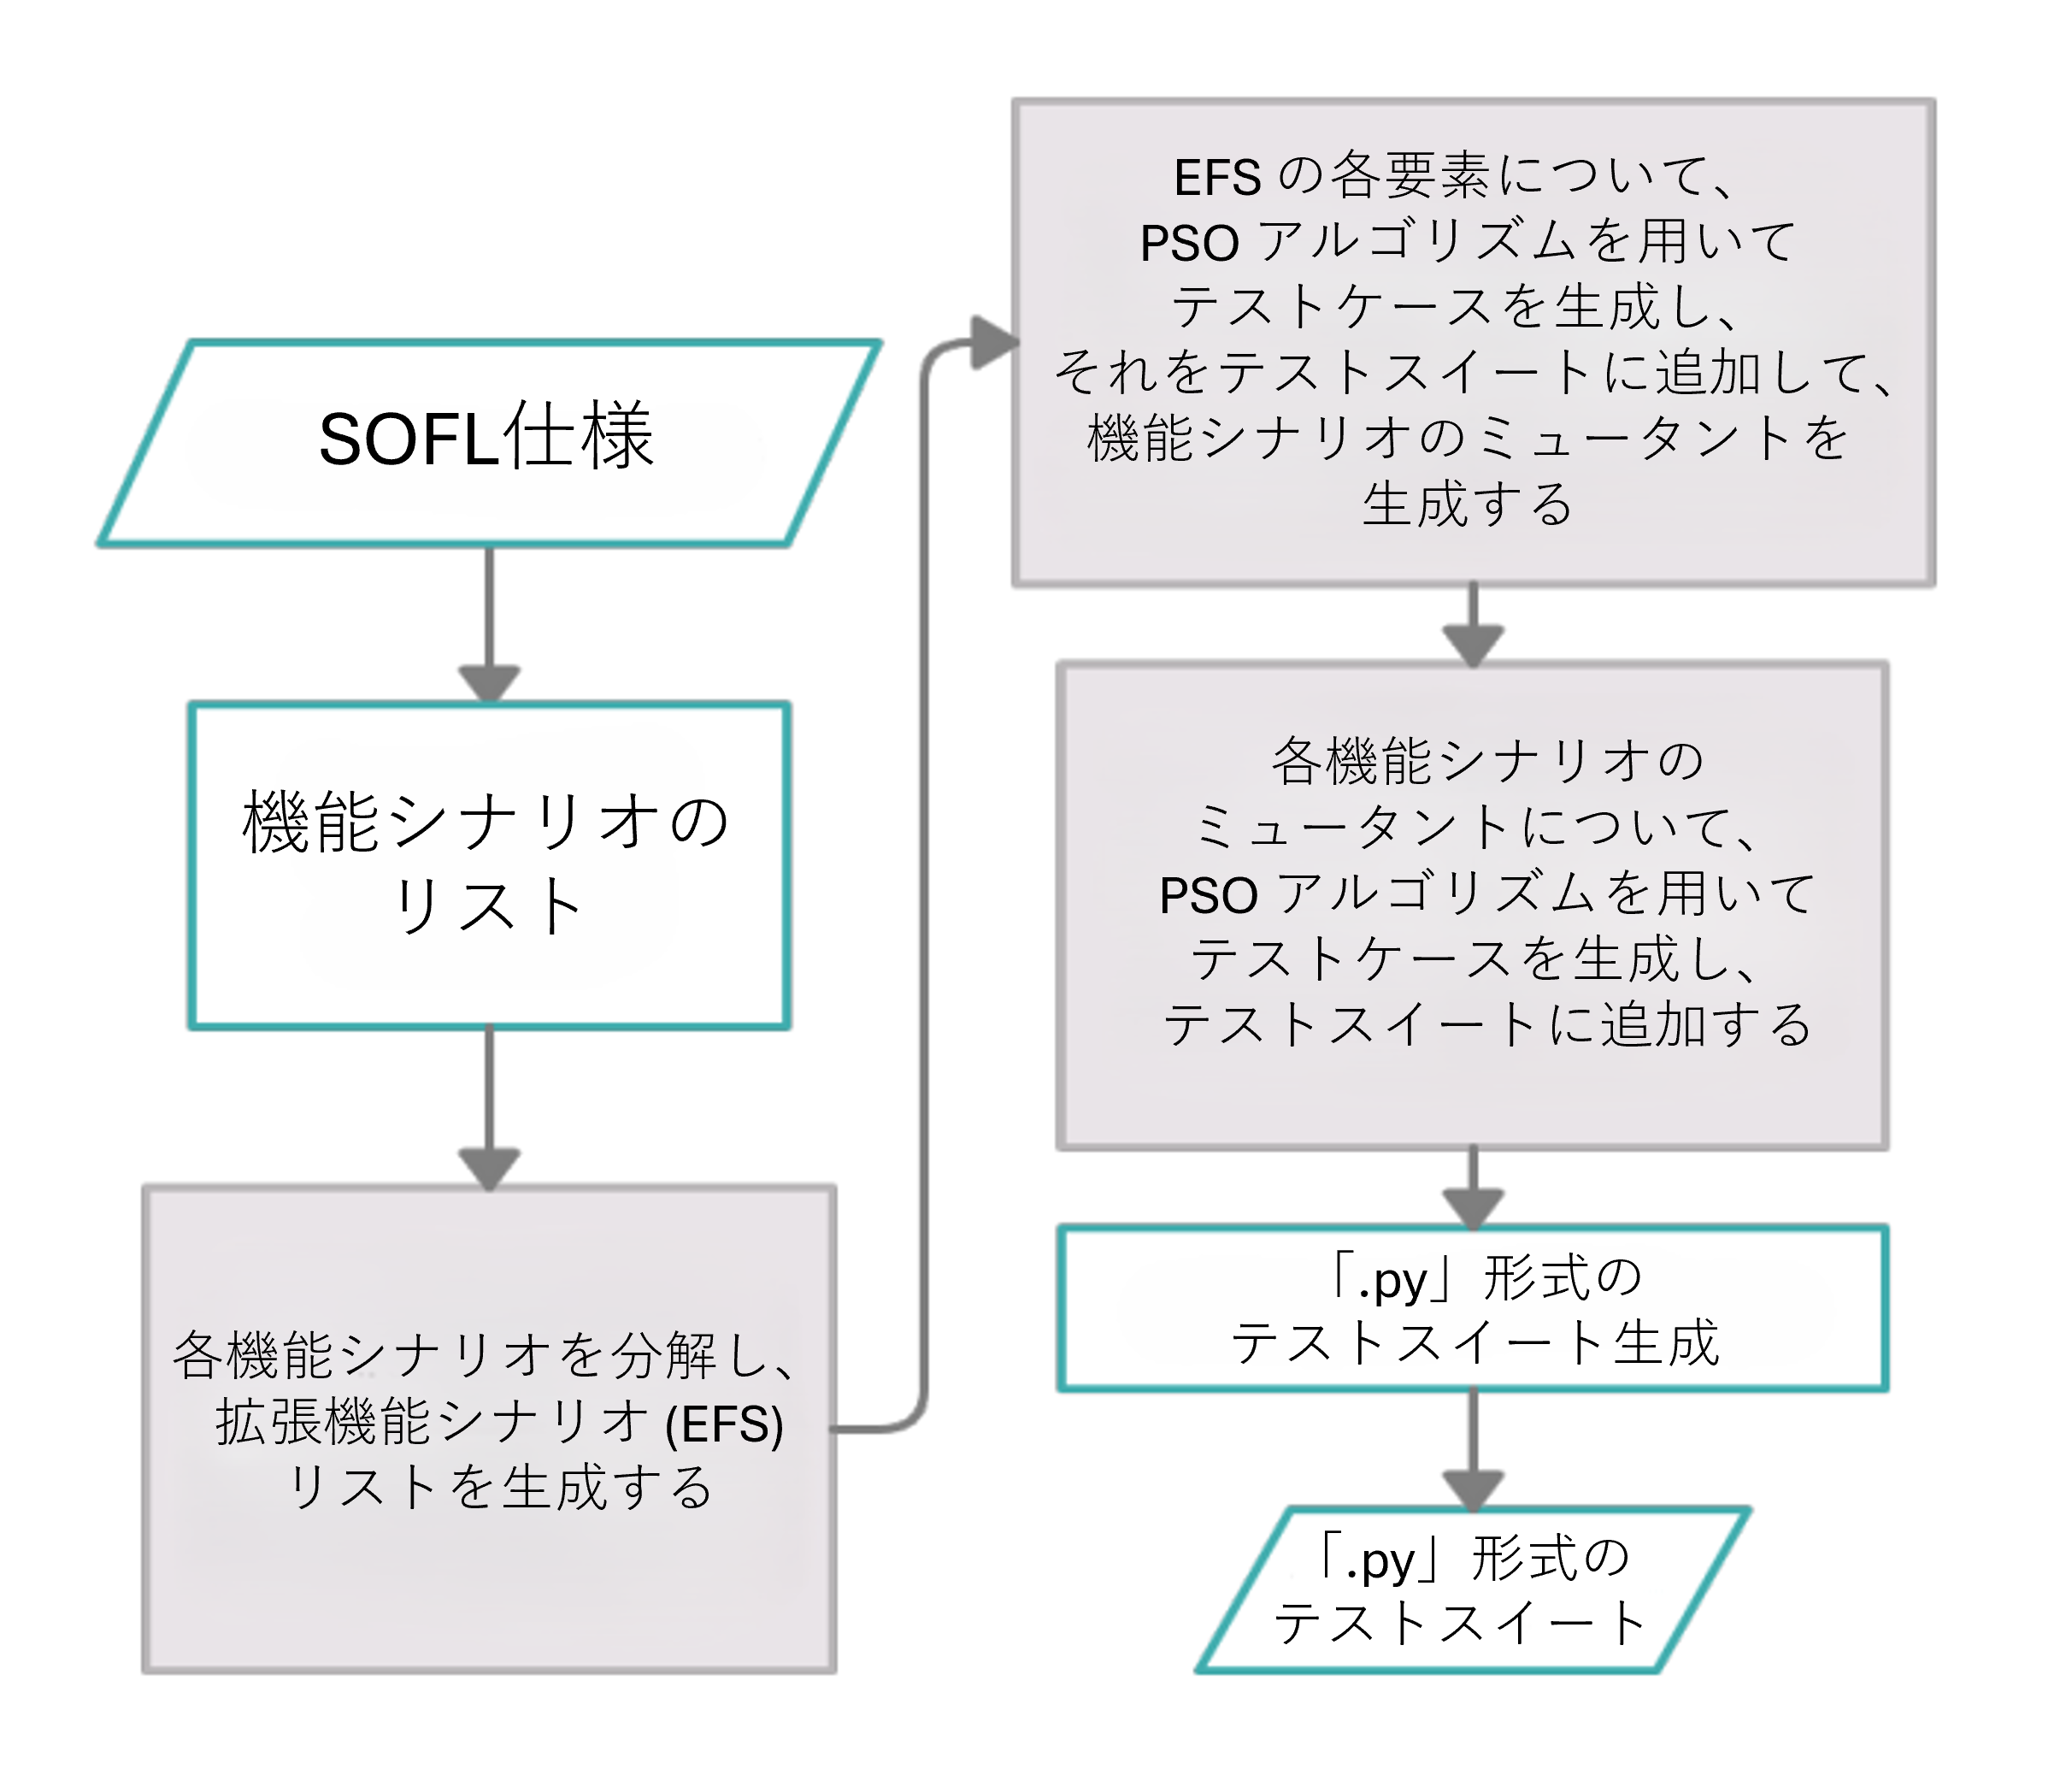
\includegraphics[width=\linewidth]{../image/Automatic_Generation_of_Test/tool_process.png}
        \caption{ツールのプロセス}
        \label{fig:tool_process}
    \end{center}
\end{figure}

\subsection{SOFL 仕様}
本ツールの機能を説明するために、最大公約数 (GCD: Greatest Common Divisor) を例として用いる。
GCD 関数の自然言語による仕様は、2つの与えられた数に対して、その最大公約数を返す関数であることを示している。

この非形式仕様を、関数が行う各動作を示す条件を特定することにより、手作業で SOFL 仕様に変換する。
DNF では、すべての可能な動作を述語で表現し、論理和の各要素がそれぞれの動作を意味している。
図\ref{fig:GCD_function}に示すように、各動作は、入力変数と出力変数を含む述語の論理積によって表現する。

\begin{figure}[tp]
    \begin{center}
        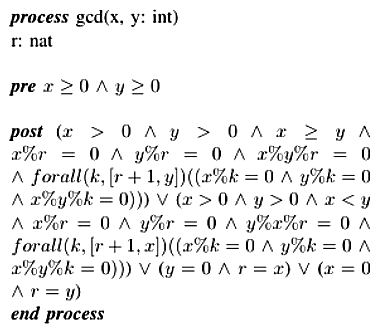
\includegraphics[width=\linewidth]{../image/Automatic_Generation_of_Test/GCD_function2.png}
        \caption{SOFL 仕様における GCD 関数}
        \label{fig:GCD_function}
    \end{center}
\end{figure}

SOFL 仕様では、事後条件は DNF による述語として記述する。
事前条件との論理積により構成する述語の要素が、1つの機能シナリオを表す。
例えば、本仕様における最初の機能シナリオである FS1 は以下の通りである:\\

FS1: $x \geq 0 \land y \geq 0 \land x > 0 \land y > 0 \land x \geq y \land x\%r = 0 \land y\%r = 0 \land x\%y\%r = 0 \land forall(k,[r+1,y])((x\%k = 0 \land y\%k = 0 \land x\%y\%k = 0))$.\\

FS1 には、テスト条件と定義条件という2つの主要な構成要素が存在する。
機能シナリオにおけるテスト条件は、ガード条件と事前条件の論理積からなる。
ガード条件は、FS1 において事前条件を除いた、入力のみに関係する部分である。
例えば、FS1 のガード条件 G1 は次のようになる:\\

G1: $x > 0 \land y > 0 \land x \geq y$.\\

また、FS1 のテスト条件 T1 は以下となる:\\

T1: $x \geq 0 \land y \geq 0 \land x > 0 \land y > 0 \land x \geq y$.\\

入力変数のデータを生成するために、テスト条件を使用する。
一方、定義条件は、FS1 において出力変数を1つ以上含む部分であり、期待出力を生成するために使用する。
例えば、FS1 の定義条件 D1 は以下のようになる:\\

D1: $x\%r = 0 \land y\%r = 0 \land x\%y\%r = 0 \land forall(k,[r+1,y])((x\%k = 0 \land y\%k = 0 \land x\%y\%k = 0))$.\\

\subsection{機能シナリオの分解}
機能シナリオにおいて、ガード条件に`$\geq$',`$\leq$',`$\neq$'といった演算子を含む場合、そのシナリオを2つのシナリオに分解する。
例えば、FS1 のガード条件には述語 $x \geq y$ が含まれており、これを $x > y$ を含むシナリオと $x = y$ を含むシナリオの2つに分解する。

本ツールは、各機能シナリオを分解し、拡張機能シナリオ (EFS) のリストを生成する。
EFS の各要素は、テストケースを生成するために用いる。
入力変数の値は、テスト条件をもとに PSO アルゴリズムを用いて導出し、出力変数の値は、定義条件をもとに PSO アルゴリズムを用いて導出する。
本ツールは、図\ref{fig:First_test_suite}に示すテストスイートを返す。

\begin{figure}[tp]
    \begin{center}
        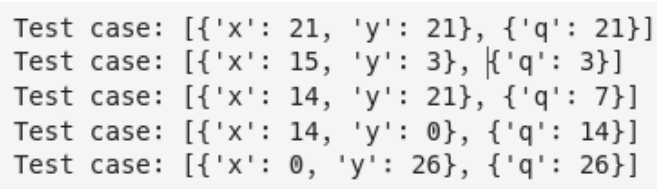
\includegraphics[width=\linewidth]{../image/Automatic_Generation_of_Test/First_test_suite.png}
        \caption{EFS より生成した最初のテストスイート}
        \label{fig:First_test_suite}
    \end{center}
\end{figure}

\subsection{テストケース生成器としての PSO アルゴリズム}
PSO アルゴリズムは、コスト関数の値を最小化することで、特定の述語を満たすデータを生成するために使用する。
本ツールは、PSO アルゴリズムを処理の2つの段階で実行する。
まず、EFS の各要素に対してテストケースを生成するために実行する。
つまり、EFS の各要素ごとに1回、PSO アルゴリズムを実行する。
次に、各述語のミューテーションに対してテストケースを生成するために実行する。
ここでは、各述語のミューテーションに対して2回 PSO アルゴリズムを使用する。
1回はテスト条件を用いて、もう1回は定義条件を用いて実行する。

\subsection{機能シナリオのミューテーション}
ミュータントを生成するために、ミューテーション操作を適用する必要がある。
このミューテーション操作は、述語 (または機能シナリオ) の構文を変更する。
本ツールは、述語内の関係演算子を変更するミューテーション操作を使用する。
例えば、`$>$'演算子を`$=$'演算子に置換する。

このミューテーション操作を機能シナリオのガード条件に適用することで、新しいガード条件を生成する。
このガード条件は、PSO アルゴリズムによって、それを満たすデータを生成するために使用する。
次に、生成した新たなデータを使用して、新たなデータに合致する機能シナリオのガード条件を探索する。
そして、合致した機能シナリオの定義条件および事後条件と、ミューテーションしたガード条件を論理積で結合する。
この結合により生成した論理式が、機能シナリオミュータントである。

各機能シナリオミュータントとPSO アルゴリズムを用いてテストケースを生成し、EFS によって生成したテストスイートに、このテストケースを追加する。
このテストスイートを、図\ref{fig:Test_suite_generated_with_functional_scenatios_mutants}に示す。

\begin{figure}[tp]
    \begin{center}
        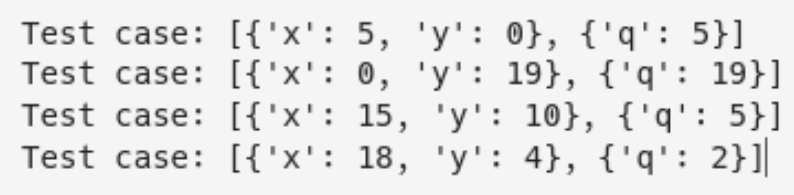
\includegraphics[width=\linewidth]{../image/Automatic_Generation_of_Test/Test_suite_generated_with_functional_scenatios_mutants.png}
        \caption{機能シナリオミュータントより生成したテストスイート}
        \label{fig:Test_suite_generated_with_functional_scenatios_mutants}
    \end{center}
\end{figure}

\subsection{Python テストファイル}
EFS および機能シナリオミュータントによって生成したテストケースを、Pythonのテストファイルに変換する。
このPythonテストファイルは、対応するPythonで記述したプログラムとともに MutPy で検証し、テストスイートの品質を評価する。


% =================  5. 結果  ====================
\section{結果}
\label{sec:result}
本研究で提案したツールを、Pythonで実装された5つの例題を用いて検証した。
3つの例題 (triangle、commission、next date) はJorgensen\cite{8}によるものであり、残りの2つ (mod、gcd) はLiu\cite{9}によるものである。
各例題に対する2種類のテストスイート $T_1$ および $T_2$ の比較結果を表\ref{tab:Mutation_score}に示す。
\begin{table}[t]
    \caption{例題のミューテーションスコアの結果}
    \label{tab:Mutation_score}
    \begin{tabular}{|c|c|c|c|c|}
        \hline
        Name      & MS($T_1$) & $\;\lvert T_1 \rvert\;$ & MS($T_2$) & $\;\lvert T_2 \rvert\;$ \\ \hline
        Next Date & 1         & 61                      & 0.95      & 13                      \\
        Mod       & 1         & 6                       & 1         & 3                       \\
        Triangle  & 1         & 59                      & 0.93      & 8                       \\
        GCD       & 1         & 9                       & 1         & 4                       \\
        Com       & 1         & 11                      & 0.93      & 3                       \\ \hline
    \end{tabular}
\end{table}
$T_1$ は、本ツールを用いて生成したテストスイートであり、$T_2$ は、もとの形式仕様における各機能シナリオに対して、テストケースを生成して作成したテストスイートである。
いずれのテストスイートも、テストケース生成器として PSO アルゴリズムを用いて生成を行った。
表\ref{tab:Mutation_score}は、それぞれのテストスイートが含むテストケースの数を示しており、$\;\lvert T_1 \rvert\;$および$\;\lvert T_2 \rvert\;$と表す。
各テストスイートが達成したミューテーションスコアは、MutPy を用いて評価し、それぞれ MS($T_1$) および MS($T_2$) と表す。
$T_2$ は平均ミューテーションスコア 0.96 を達成し、$T_1$ は平均ミューテーションスコア 1 を達成していることが分かる。

% =================  6. 結論と今後の課題  ====================
\section{結論と今後の課題}
\label{sec:conclusion_and_future_work}
本研究では、PSO アルゴリズムがテストケース生成器として有効であることを示した。
これは、形式言語と組み合わせて PSO アルゴリズムをテスト目的で用いた初めての試みである。
このアルゴリズムは、あらゆる機能シナリオに対してテストケースを見つけ出すことに成功した。
本ツールは、ただテストスイートを自動で生成するだけでなく、SOFL 仕様から形式的かつ効果的にテストスイートを生成することができる。
また、機能シナリオミュータントから生成したテストケースを追加することでテストスイートを拡張でき、実験結果が示すように、ミュータントスコア 1 を達成するテストスイートを生成した。

本ツールのさらなる拡張および、本ツールと他ツールの比較評価が、今後の課題として挙げられる。

\section*{訳者の感想}
形式仕様からのテストケース生成に関する手法の中で、記号実行を用いたもの以外の手法を知りたくて、本論文を読んだ。
PSO アルゴリズム (群知能) を用いて、テストケース生成を行うという手法を知り、参考になった。
また、SOFL に関しては、VDM に近しい部分も多く、SOFL を用いた手法は、VDM を扱うにあたって参考になる部分が多そうだと感じた。
これからは、SOFL を用いた手法の調査も行いたい。

加えて、本論文ではミューテーションテストに関する記述もあった。
実際に、形式仕様からミュータントを用いたテストケースを生成しており、
形式仕様とミューテーションテストの組み合わせに関して、実現可能性を感じた。
ミュータントを用いたテストケース生成は、テストスイートの品質向上に有効な手段だと考えるため、BWDM の拡張方針の一案として検討できると考えた。
しかし、本論文で実際に生成していたテストケースの内容は、現在の BWDM でも生成できそうだと感じた。
BWDM にミュータントからテストケースを生成する機能を適用することにより、実際にテストスイートの品質は向上するのかという部分も含めて、さらなる調査の必要性を感じた。

論文の内容に関しては、PSO アルゴリズム、SOFL、ミューテーションテストなど、形式仕様を用いたテストケース生成を行うにあたり、参考になる技術が多く含まれていた。
しかし、\ref{sec:result}章、\ref{sec:conclusion_and_future_work}章の内容が薄かったことが残念である。
本論文で示されている結果は、ミューテーションテストを行っていなくてもミューテーションスコアがすでに高く、ミューテーションテストの効果を十分に把握するには至らないと感じた。
また、今後の課題で述べられている通り、他ツールとの比較も行われていないため、実際に提案している手法がどれだけ有効なのかが一側面からしか述べられておらず、
この手法の強みと欠点が分からないと感じた。
本論文の評価で使用している問題の一部は参照できそうなので、実際に BWDM に適用して比較してみたい。

\begin{thebibliography}{99}
    \bibitem{1} M. W. W. Matt Staats and M. P. Heimdahl. 2011. “Better testing through oracle selection,” in ICSE '11.
    \bibitem{2} Rashmi Rekha Sahoo, Mitrabinda Ray. 2020. ``PSO based test case generation for critical path using improved combined fitness function,” Journal of King Saud University Computer and Information Sciences.
    \bibitem{3} S. Liu and S. Nakajima. 2010. “A decompositional approach to automatic test case generation based on formal specifications,” Fourth IEEE International Conference on Secure Software Integration and Reliability Improvemet.
    \bibitem{4} A. P. Mathur. 2013. ``Foundations of software testing,” Pearson.
    \bibitem{5} Shaoying Liu and Yong Sun. 1995. ``Structured methodology+object-oriented methodology+formal methods: methodology of SOFL,” proceedings of First IEEE International Conference on Engineering of Complex Computer Systems. pp. 137-144.
    \bibitem{6} Cencen Li, Mo Li, Shaoying Liu, Shin Nakajima. 2012. ``Structured Object-Oriented Formal Language,” Lecture Notes in Computer Science 7787.
    \bibitem{7} J. Kennedy and R. Eberhart. 1995. ``Particle swarm optimization,” Proceedings of ICNN'95 - International Conference on Neural Networks, pp. 1942-1948 vol.4.
    \bibitem{8} Paul C. Jorgensen. 2013. ``Software Testing: a Craftman's approach,” CRC Press, fourth edition.
    \bibitem{9} R. Wang, Y. Sato and S. Liu. 2019. ``Specification-based Test Case Generation with Genetic Algorithm,” IEEE Congress on Evolutionary Computation (CEC), pp. 1382-1389.
    \bibitem{10} Aichernig B.K., Lorber F., Ni\v{c}kovi\'c D.. 2013. ``Time for Mutants — Model-Based Mutation Testing with Timed Automata,” In: Veanes M., Vigan\'o L. (eds) Tests and Proofs. Lecture Notes in Computer Science, vol. 7942. Springer, Berlin, Heidelberg.
    \bibitem{11} Fraser, Gordon and Wotawa, Franz. 2006. ``Using ModelCheckers for Mutation-Based Test-Case Generation, Coverage Analysis and Specification Analysis,” 16. 10.1109/ICSEA.2006.75
    \bibitem{12} Gustavo Carvalho, Diogo Falc\~ao, Fl\'avia Barros, Augusto Sampaio, Alexandre Mota, Leonardo Motta, Mark Blackburn. 2014. ``NAT2TESTSCR: Test case generation from natural language requirements based on SCR specifications,” Vol. 95, pp. 275-297, ISSN 0167-6423.
    \bibitem{13} Larsen, K., Lorber, F., Nielsen, B., and Nyman, U. 2017. ``Mutation-Based Test-Case Generation with Ecdar,” IEEE International Conference on Software Testing, Verification and Validation Workshops (ICSTW), pp 319-328.
    \bibitem{14} Wang, Rong, Yuji Sato, and Shaoying Liu. 2021. ``Mutated Specification-Based Test Data Generation with a Genetic Algorithm,” Mathematics 9, no. 4: 331.
    \bibitem{15} Nayak, N., and Mohapatra, D. P.. 2010. ``Automatic Test Data Generation for Data Flow Testing Using Particle Swarm Optimization,” Contemporary Computing, 1-12.
\end{thebibliography}

\end{document}